Auf Basis der verfeinerten Dimensionierung des Holmes mithilfe von ELAMX und der Beulabschätzung, soll nun ein CAD-Modell des Flügels erstellt werden. Als Grundlage dient eine unvollständige technische Zeichnung der Profilkontur, aus der exakt entnommen werden kann, dass das Profil ohne die Hochauftriebselemente oder Querruder $ 172mm $ tief ist und eine Profildicke von $ 37,5mm $ aufweist. Aus den bekannten Längenangangaben kann der Maßstab der gedruckten Zeichnung zu $ 1:1,039 $ berechnet werden. Mithilfe eines Rechtecks, das die Kontur gerade umschließt, können weitere Punkte auf der Kontur des Profils ermittelt werden. Im CAD-Programm werden Tangentenbögen von Punkt zu Punkt gelegt, um die Kontur hinreichend glatt anzunähern.\\


\noindent In den Bereichen oberhalb und unterhalb des Holms soll die Haut nicht in Sandwich-Bauweise ausgeführt sein. Für die Auslegung des Holms wurde davon ausgegangen, dass eine Dicke des Verbundmaterials der Haut von $ 0,75mm $ ausreichend ist. Zunächst wird davon ausgegangen, dass für die Haut das Gewebe Interglas 90070 verwendet wird, das ein Flächengewicht von $ 80\frac{g}{m^{2}} $ aufweist. Die Begründung dieser Annahme liegt in den annähernd gleichen Anteilen der Fasern in Kette- und Schußrichtung. Da die Haut des Flügels insbesondere die aus der Torsion resultierende Schubspannung aufnehmen soll, bietet sich die Verwendung eines Gewebes in Leinwandbindung mit diesen Eigenschaften an. Nach Gleichung ~\ref{gurtlagen} entsprechen $ 9 $ Lagen dieses Gewebes der angenommenen Hautdicke. Für die Vorauslegung der Haut erscheint dies ausreichend. Sollten weniger Lagen für die Haut benötigt werden, kann der entstehende Freiraum zwischen den Gurten und der Haut aufgefüllt werden. Um die Hautdicke von $ 0,75mm $ im Bereich der Gurte zu berücksichtigen, wird ein Offset von dieser Breite nach innen gerichtet.\\
\noindent Der zu Beginn des Abschnitts ~\ref{GurtDim} dimensionierte Holm mit rechteckigen Gurtquerschnitten, $ b=28mm $ und $ h_{a}=36mm $ wird nun so auf die Kontur des Profils gelegt, dass die Überdeckung der Gurte mit der umgebenden Haut möglichst gering ausfällt. Dann wird die Höhe $ h_{a} $ an den örtlichen inneren Abstand der oberen und unteren Haut auf $ \tilde{h_{a}}=35,8mm $ angepasst. Der rechteckige Querschnitt der Gurte wird mithilfe eines Offsets von $ \tilde{h}=1,941mm $ der Kontur der Haut angepasst. Diese Anpassungsmaßnahmen senken das Flächenträgheitsmoment leicht. Das resultierende Flächenträgheitsmoment $ \tilde{I_{x}} $ lässt sich aufgrund der komplexen Querschnittsgeometrie der Gurte nur mit dem CAD-Programm exakt bestimmen. 
\begin{figure}
	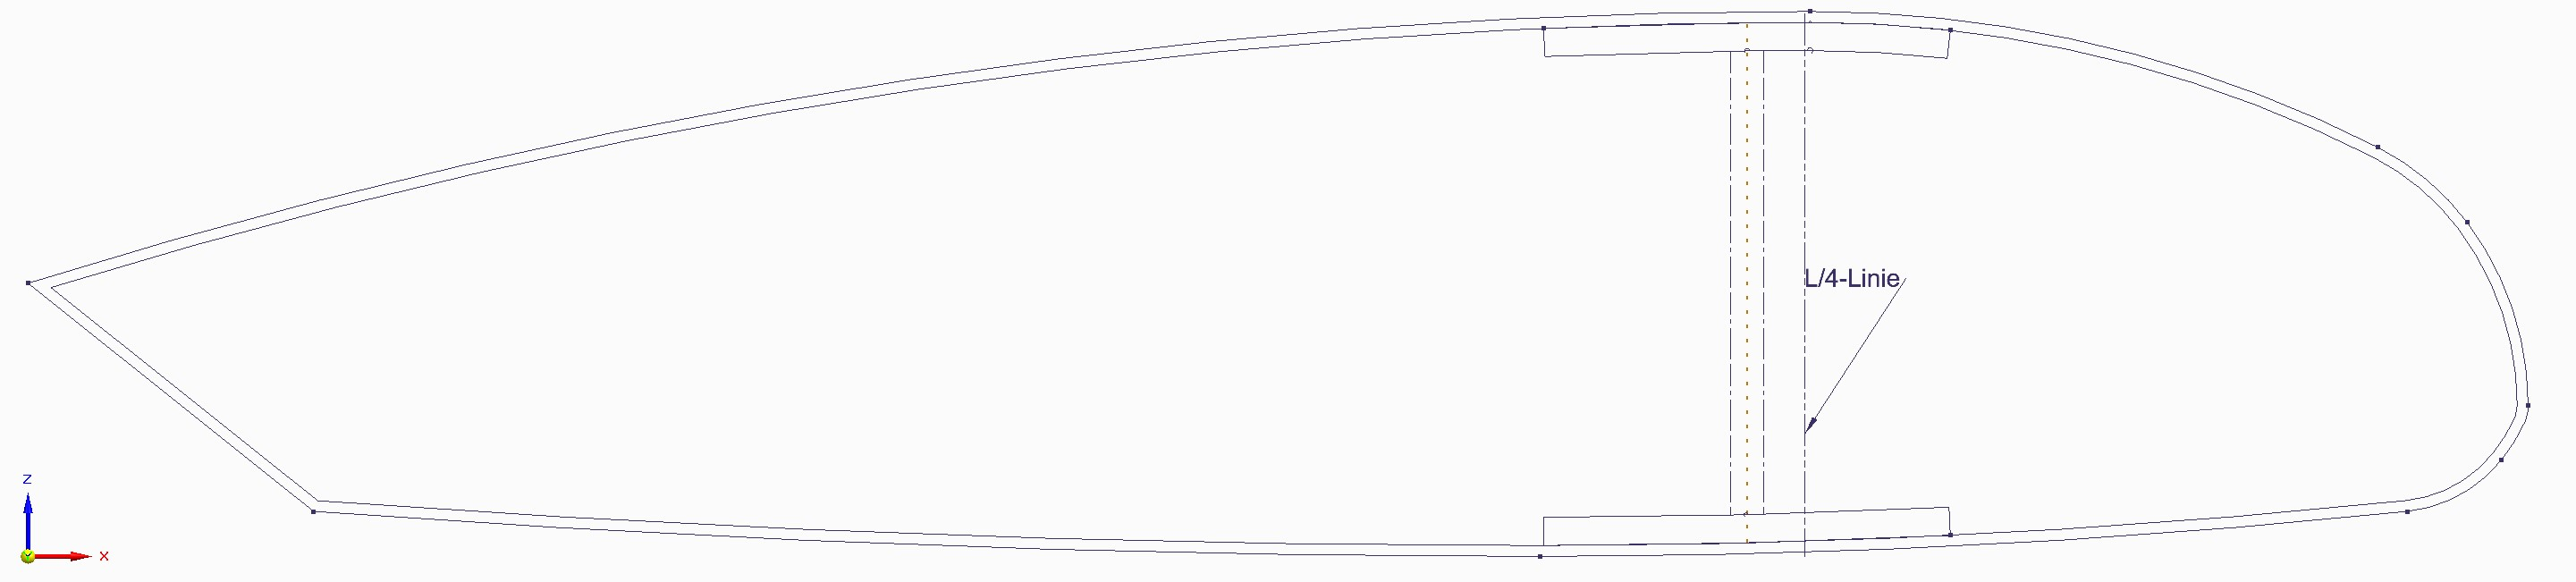
\includegraphics[width=1.0\textwidth]{Bilder/Kontur.jpg}
	\caption{Haut und Gurte nach dem ersten Schritt der Konstruktion in Solid Edge.}
	\label{fig: Kontur}
\end{figure} 
Der Vergleich mit dem erforderlichen Flächenträgheitsmoment zeigt, dass die angepasste Geometrie der Gurte die Steifigkeitsbedingung (vergleiche Beziehung ~\ref{IVergleich}) erfüllt. Die Haut konstanter Dicke und die Gurte im ersten Schritt der Konstruktion werden durch Abbildung ~\ref{fig: Kontur} veranschaulicht. Zusätzlich zeigt die Abbildung die ungefähre Lage der L/4-Linie. Diese wurde mithilfe einer vorhandenen Hilfsansicht der Tragfläche inklusive der Hinterkantenklappen und des Vorflügels, beide im eingefahrenen Zustand, ermittel. In der Hilfsansicht wird die abgebildete Länge des mittleren auszulegenden Teils der Tragfläche gemessen. Der Maßstab der Hilfsansicht bezüglich des Modellmaßstabes wird zu 1:2,529 berechnet. Diese Kenntnis ermöglicht die Berechnung des Abstandes der L/4-Linie zur Vorderkante der Haupttragfläche, der $ 42,2mm $ beträgt und besonders für die Berechnung der Torsion ausschlaggebend ist.\\

\begin{figure}
	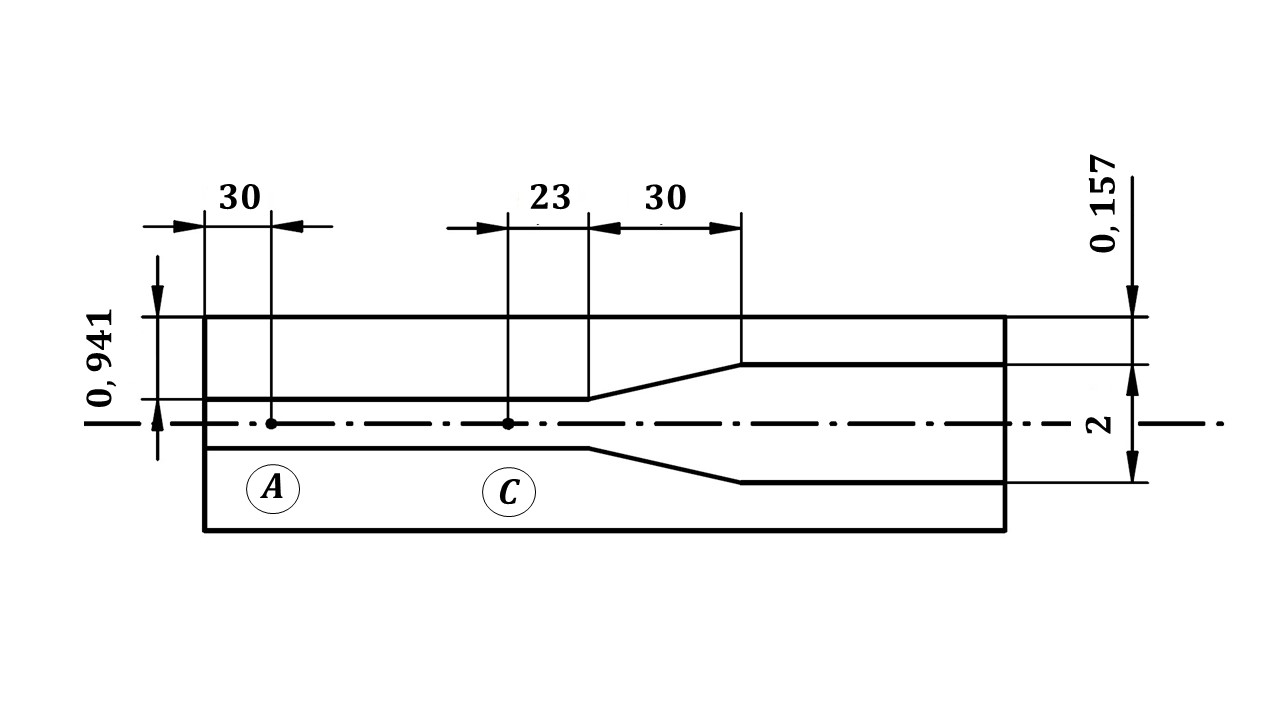
\includegraphics[width=1.0\textwidth]{Bilder/StegPrinzip.jpg}
	\caption{Prinzipskizze der Sandwichstruktur im Steg.}
	\label{fig: Steg}
\end{figure}

\noindent Im nächsten Schritt wird die Kontur der zwei Stegseiten und des Schaumes in einer weiteren Skizze über der Kontur der Gurte gezeichnet. Die vielschichtigen Skizzen erlauben den Bezug von Bauteilkanten aufeinander und erleichtern die spätere Extrusion der einzelnen Komponenten. So kann sichergestellt werden, dass in jeder Komponente der Bezug auf die umgebenden Tangentenbögen der Haut gewahrt bleibt. Die Konstruktion des Steges und des Schaumes erfordert auch die Berücksichtigung der verschieden belegten Unterteilungen des Stegs. Während der innere Teil des Stegs, am inneren freien Ende beginnend und $ 23mm $ über die Aufnahme der Querkraftbolzen an Punkt C hinweggehend, gemäß der Dimensionierung mithilfe des Laminatrechners mit 24 Lagen, aufgeteilt zu jeweils zwölf Lagen auf beiden Seiten des Schaums belegt wird, soll der gesamte äußere Teil mit nur insgesamt vier Lagen gleichmäßig verteilt belegt werden. Es bietet sich an, die vier Lagen des äußeren Teils über die gesamte Holmlänge zu erstrecken. Die 20 verstärkenden Lagen enden $ 23mm $ hinter Punkt C in einem sanften Übergang mit einer Länge von 30mm. Der dünn belegte Teil wird durch einen $ 2mm $ breiten Schaumkern vor dem Beulen geschützt, der zum dick belegten Teil hin entsprechend schmaler wird. Das innere freie Ende wird auf eine Länge von $ 30mm $ im Abstand vom Mittelpunkt des Lagers A abgeschätzt. Abbildung ~\ref{fig: Steg} veranschaulicht den prinzipiellen Aufbau qualitativ.


